\documentclass[12pt]{article}
\usepackage[T1]{fontenc}
\usepackage[T1]{polski}
\usepackage[utf8]{inputenc}
\newcommand{\BibTeX}{{\sc Bib}\TeX}
\usepackage{graphicx}
\usepackage{amsfonts}

% OWN PACKAGE - VERY IMPORTANT %
\usepackage{float}
%%%%%%%%%%%%%%%%%%%%%%%%%%%%%%%%%

\setlength{\textheight}{21cm}


\title{{\bf Zadanie nr 4 - Przekształcenie Fouriera, Walsha-Hadamarda,
kosinusowe i falkowe, szybkie algorytmy}\linebreak
    Cyfrowe Przetwarzanie Sygnałów}
\author{Jan Karwowski 216793 \and Kamil Kowalewski 216806}
\date{data oddania zadania 13.05.2020r}

\begin{document}
    \clearpage\maketitle
    \thispagestyle{empty}
    \newpage
    \setcounter{page}{1}
%--------------------------------------------------------------------------------------%
    \section{Cel zadania} {
        Celem zadania jest zapoznanie się z operacjami transformacji sygnałów dyskretnych
        przy użyciu wybranych metod oraz zaimplementowanie ww. operacji transformacji
        w programie z zadania trzeciego.
    }
%--------------------------------------------------------------------------------------%

    \section{Wprowadzenie} \label{intro}{
        Na podstawie instrukcji ze strony przedmiotu~\cite{instrukcja}
        do programu z zadania trzeciego zostały dodane funkcjonalności
        do odczytu i zapisu sygnałów o wartościach zespolonych oraz
        możliwości rysowania wykresów sygnałów dyskretnych o
        wartościach zespolonych w postaci dwóch wykresów o wspólnej
        dziedzinie. Wykresy są umieszczone jeden nad drugim oraz
        zostało przyjęte założenie, że sygnały zespolone będą tylko
        wynikiem transformacji Fouriera, więc będą prezentować funkcje
        w dziedzinie częstotliwości.
        Zostały zapewnione dwa tryby wyświeltania wykresu:
        \begin{itemize}
            \item (W1) – górny wykres prezentuje część rzeczywistą
                amplitudy w funkcji częstotliwości, a wykres dolny
                część urojoną
            \item (W2) – górny wykres prezentuje moduł liczby
                zespolonej, a dolny argument liczby w funkcji
                częstotliwości
        \end{itemize}
        Ponadto zostały zaimplementowane transformacje przedstawione
        poniżej: 
        \begin{itemize}
            \item dyskretna transformacja Fouriera - algorytm z
                definicji o złożoności O($N^2$), gdzie wyliczenie
                każdej próbki wyniku wymaga wymnożenia i zsumowania
                wszystkich próbek sygnału wejściowego przez
                odpowiednie, wyliczane na bieżąco wsþółczynniki
            \item dyskretna transformacja Fouriera - algorytm szybki w
                miejscu (\emph{in situ}) z decymacją w dziedzinie
                czasu (DIT FFT) o złożoności O(Nlog(N)), nie wymaga
                alokacji dodatkowej pamięci na bufor próbek podczas
                obliczeń, ponadto wszystkie współczynniki są wyliczone
                przed obliczeniami w tablicy o długości równej połowy
                długości bufora próbek
            \item dyskretna transformacja Fouriera - algorytm szybki
                rekurencyjny z decymacją w dziedzinie czasu (DIT FFT),
                gdzie złożoność O(Nlog(N)) jest uzyskana poprzez
                dzielenie ciągu próbek na połowy, ale każdy krok
                rekurencji (każdy podział) wymaga alokacji nowej
                pamięci, współczynniki są wyliczane na bieżąco
            \item dyskretna transformacja kosinusowa typu drugiego -
                algorytm z definicji
            \item dyskretna transformacja kosinusowa typu drugiego -
                algorytm szybki, oparty o FFT
            \item dyskretna transformacja Walsha-Hadamarda - algorytm z
                definicji
            \item dyskretna szybka transformacja Walsha-Hadamarda -
                algorytm szybki
            \item dyskretna transformacja falkowa Daubechies czwartego
                rzędu (DB4), jeden poziom transformacji, algorytm
                oparty o macierz współczynników
        \end{itemize}
    }
    \newpage
%--------------------------------------------------------------------------------------%
    \section{Materiały i metody} {
        Pierwszym krokiem w czasie dokonywania eksperymentów było wygenerowanie trzech sygnałów
        sinusoidalnych. Ich równania zostały przedstawione poniżej:
        \begin{figure}[H]
            \label{wzory}
            \centering
            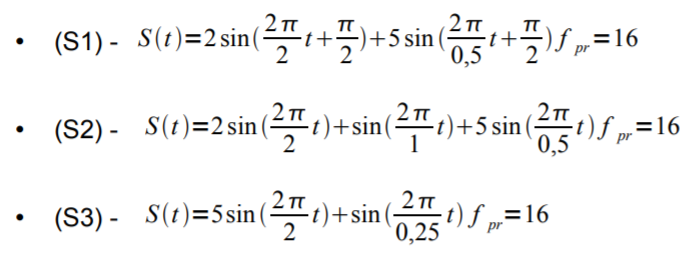
\includegraphics[width=0.7\textwidth]{img/theory/equations.png}
        \end{figure}
        Następnie zostały przeprowadzone dla każdego z nich transformaty przedstawione poniżej:
        \begin{enumerate}
            \item Dyskretna tranformacja Fouriera z definicji
            \item Dyskretna tranformacja Fouriera wariant szybki in situ
            \item Dyskretna tranformacja Fouriera wariant szybki rekurencyjny
            \item Transformacja kosinusowa z definicji
            \item Transformacja kosinusowa wariant szybki
            \item Transformacja Walsha-Hadamarda z definicji
            \item Transformacja Walsha-Hadamarda wariant szybki
            \item Transformacja falkowa wariant DB4
        \end{enumerate}

        Dla wszystkich transformat dokonaliśmy rekonstrukcji sygnału
        sposobem interpolacji pierwszego rzędu w celu uzyskania
        wykresów liniowych zamiast wykresów punktowych dla lepszego
        zobrazowania wyników.\\

        Wyniki transformat zostały przedstawione poniżej łącznie z wykresami sygnałów oznaczonych
        symbolami S1, S2, S3. 
    }
    \newpage
%--------------------------------------------------------------------------------------%
    \section{Eksperymenty i wyniki} {

        \subsection{Sygnał S1} {

            \begin{figure}[H]
                \centering
                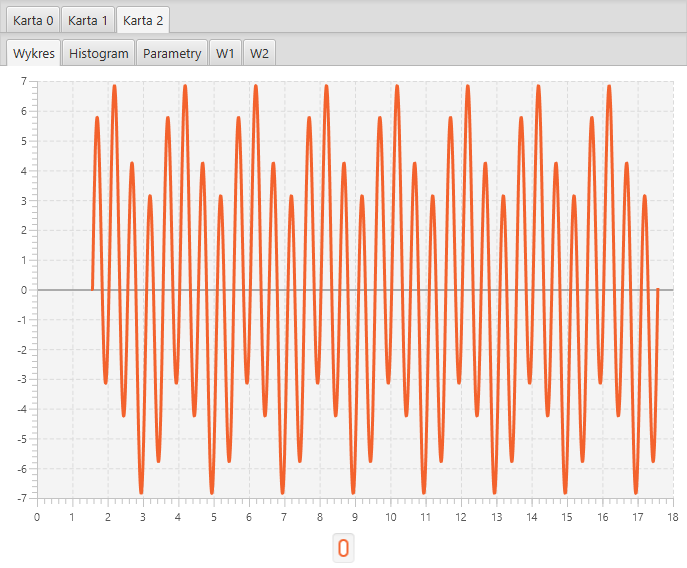
\includegraphics[width=\textwidth]{img/result/s1/data_134333.png}
                \caption{Wykres sygnału S1}
            \end{figure}
            \newpage

            \subsubsection{Dyskretna tranformacja Fouriera z definicji} {

                \begin{figure}[H]
                    \centering
                    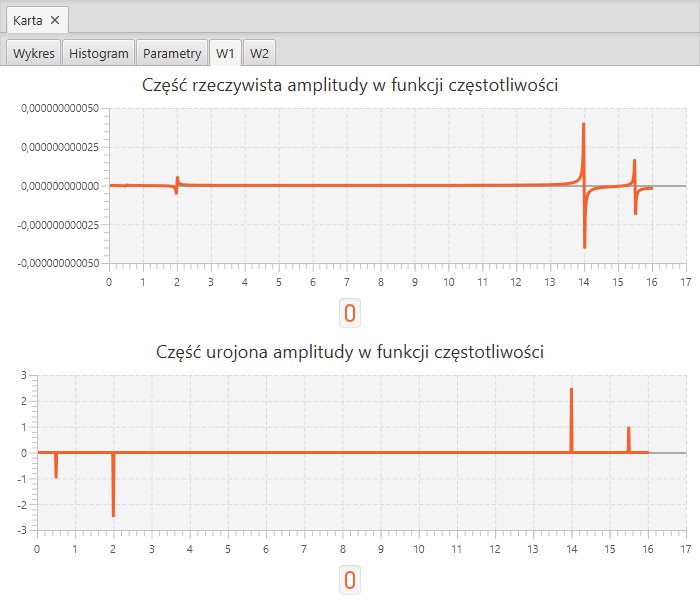
\includegraphics[width=0.65\textwidth]{img/result/s1/01/W1_draw_1_sinus_sampling_trans_s1_data_205616.png}
                    \caption{Wykresy}
                \end{figure}

                \begin{figure}[H]
                    \centering
                    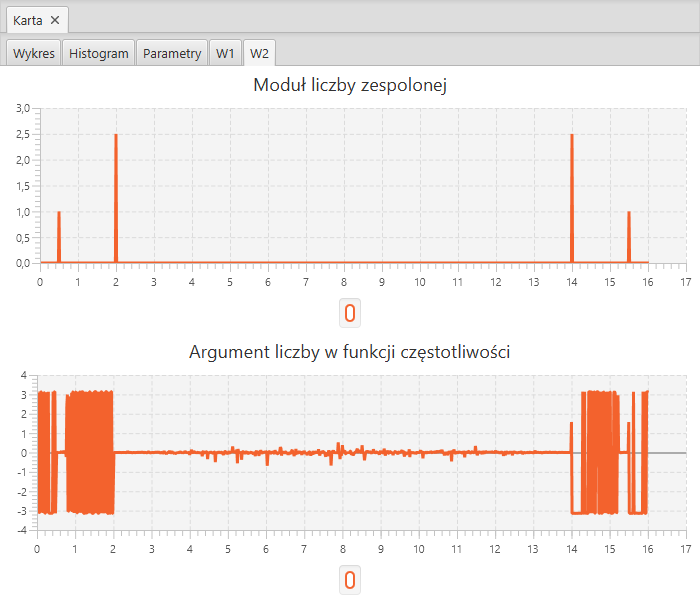
\includegraphics[width=0.65\textwidth]{img/result/s1/01/W2_draw_1_sinus_sampling_trans_s1_data_205617.png}
                    \caption{Wykresy}
                \end{figure}

                Czas wykonania obliczeń (s): 0.71
            }
            \newpage

            \subsubsection{Dyskretna tranformacja Fouriera wariant szybki in situ} {

                \begin{figure}[H]
                    \centering
                    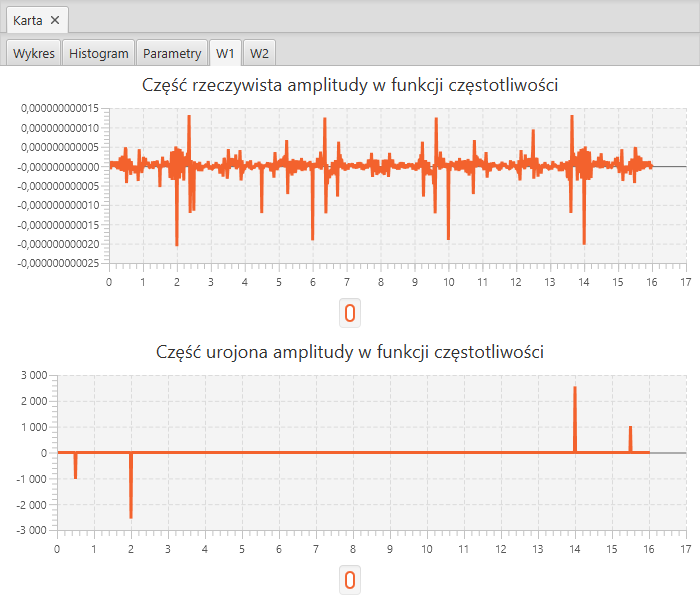
\includegraphics[width=0.65\textwidth]{img/result/s1/02/W1_draw_2_sinus_sampling_trans_s1_data_205623.png}
                    \caption{Wykresy}
                \end{figure}

                \begin{figure}[H]
                    \centering
                    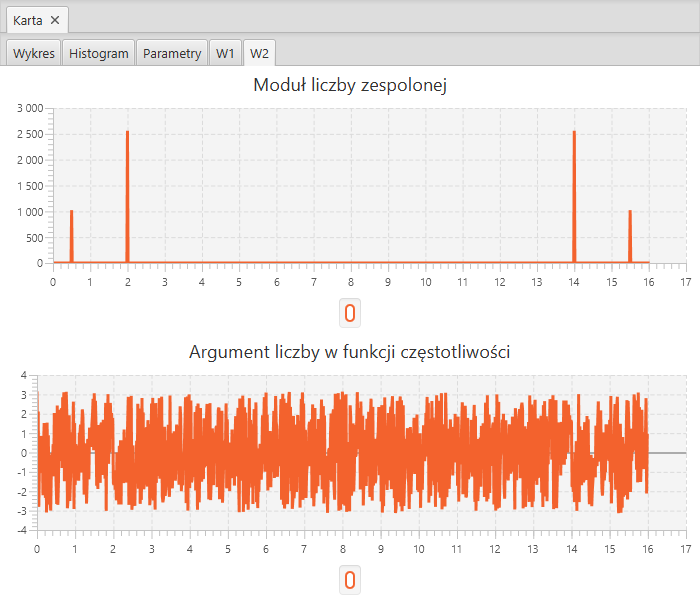
\includegraphics[width=0.65\textwidth]{img/result/s1/02/W2_draw_2_sinus_sampling_trans_s1_data_205624.png}
                    \caption{Wykresy}
                \end{figure}

                Czas wykonania obliczeń (s): 0.057
            }
            \newpage

            \subsubsection{Dyskretna tranformacja Fouriera wariant szybki rekurencyjny} {

                \begin{figure}[H]
                    \centering
                    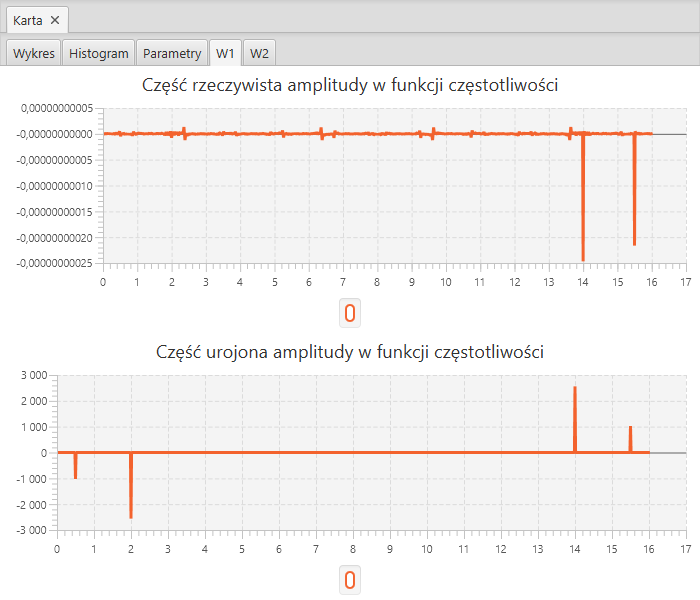
\includegraphics[width=0.65\textwidth]{img/result/s1/03/W1_draw_3_sinus_sampling_trans_s1_data_205632.png}
                    \caption{Wykresy}
                \end{figure}

                \begin{figure}[H]
                    \centering
                    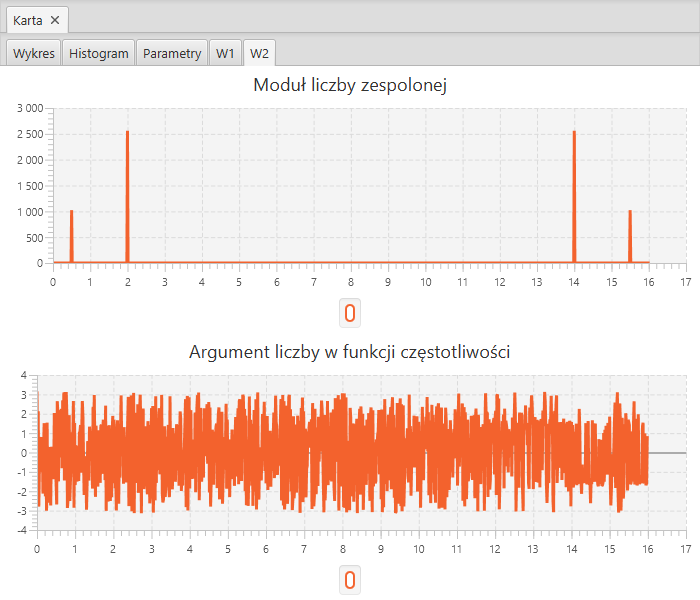
\includegraphics[width=0.65\textwidth]{img/result/s1/03/W2_draw_3_sinus_sampling_trans_s1_data_205633.png}
                    \caption{Wykresy}
                \end{figure}

                Czas wykonania obliczeń (s): 0.96
            }
            \newpage

            \subsubsection{Transformacja kosinusowa z definicji} {

                \begin{figure}[H]
                    \centering
                    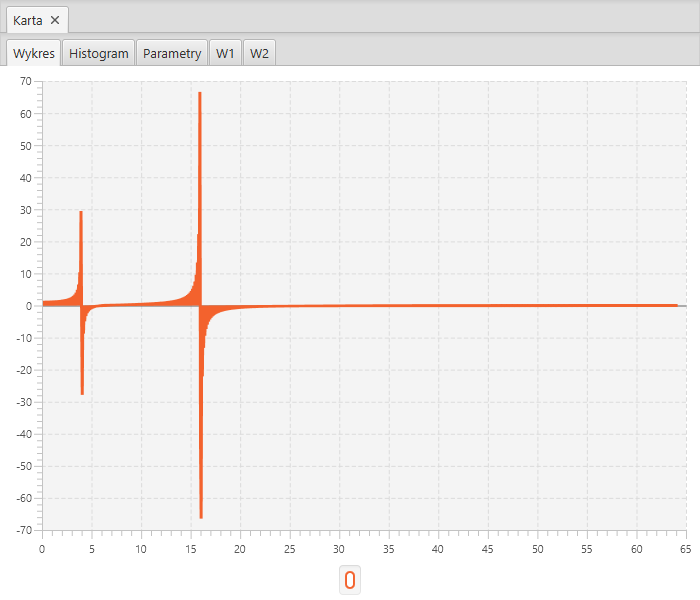
\includegraphics[width=\textwidth]{img/result/s1/04/data_draw_4_sinus_sampling_trans_s1_data_205648.png}
                    \caption{Wykresy}
                \end{figure}

                Czas wykonania obliczeń (s): 0.114
            }
            \newpage

            \subsubsection{Transformacja kosinusowa wariant szybki} {

                \begin{figure}[H]
                    \centering
                    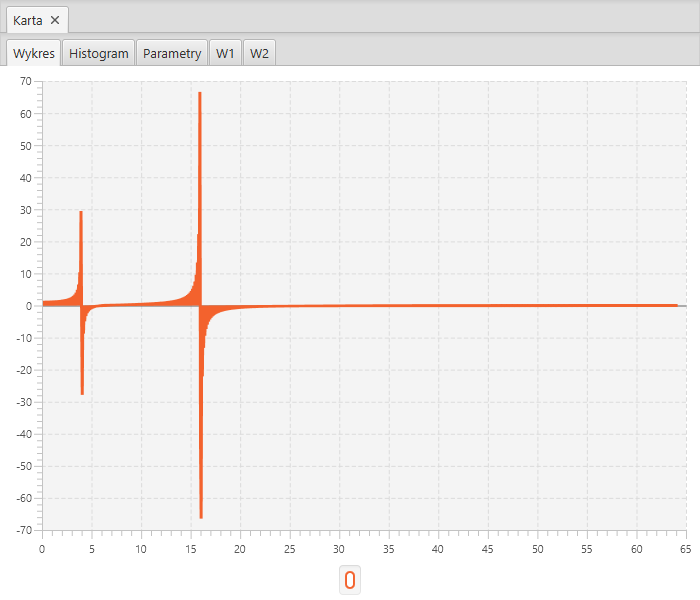
\includegraphics[width=\textwidth]{img/result/s1/05/data_draw_5_sinus_sampling_trans_s1_data_205702.png}
                    \caption{Wykresy}
                \end{figure}

                Czas wykonania obliczeń (s): 0.082
            }
            \newpage

            \subsubsection{Transformacja Walsha-Hadamarda z definicji} {

                \begin{figure}[H]
                    \centering
                    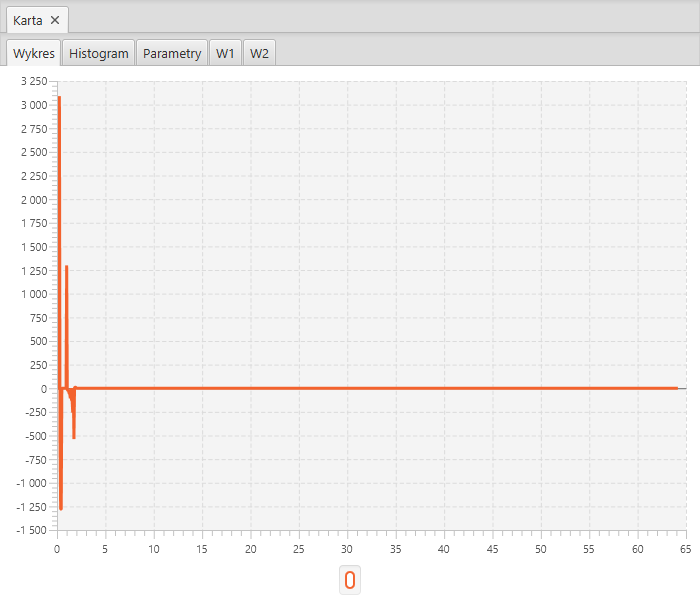
\includegraphics[width=\textwidth]{img/result/s1/06/data_draw_6_sinus_sampling_trans_s1_data_205710.png}
                    \caption{Wykresy}
                \end{figure}

                Czas wykonania obliczeń (s): 0.033
            }
            \newpage

            \subsubsection{Transformacja Walsha-Hadamarda wariant szybki} {

                \begin{figure}[H]
                    \centering
                    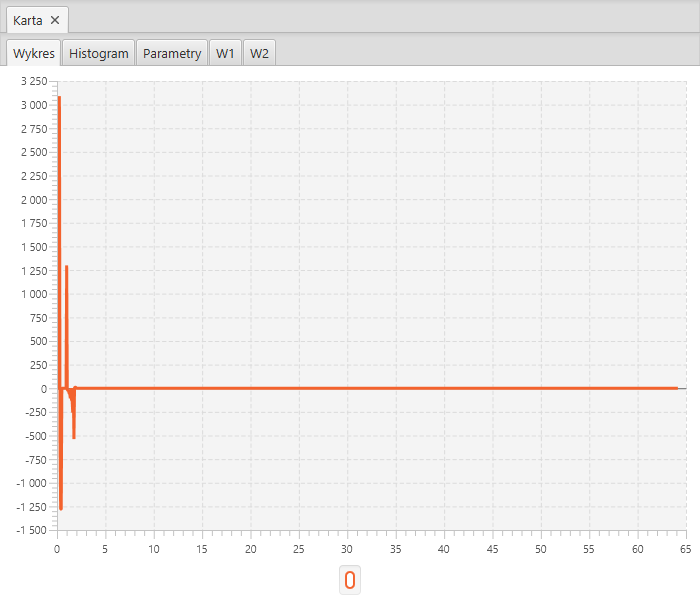
\includegraphics[width=\textwidth]{img/result/s1/07/data_draw_7_sinus_sampling_trans_s1_data_205719.png}
                    \caption{Wykresy}
                \end{figure}

                Czas wykonania obliczeń (s): 0.001
            }
            \newpage

            \subsubsection{Transformacja falkowa wariant DB4} {

                \begin{figure}[H]
                    \centering
                    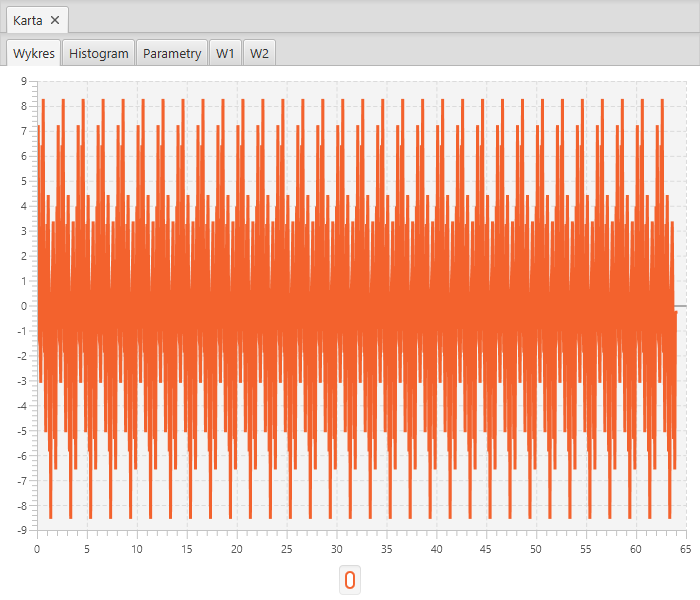
\includegraphics[width=\textwidth]{img/result/s1/08/data_draw_8_sinus_sampling_trans_s1_data_205730.png}
                    \caption{Wykresy}
                \end{figure}

                Czas wykonania obliczeń (s): 0.001
            }
            \newpage

        }
        \newpage
%--------------------------------------------------------------------------------------%
        \subsection{Sygnał S2} {

            \begin{figure}[H]
                \centering
                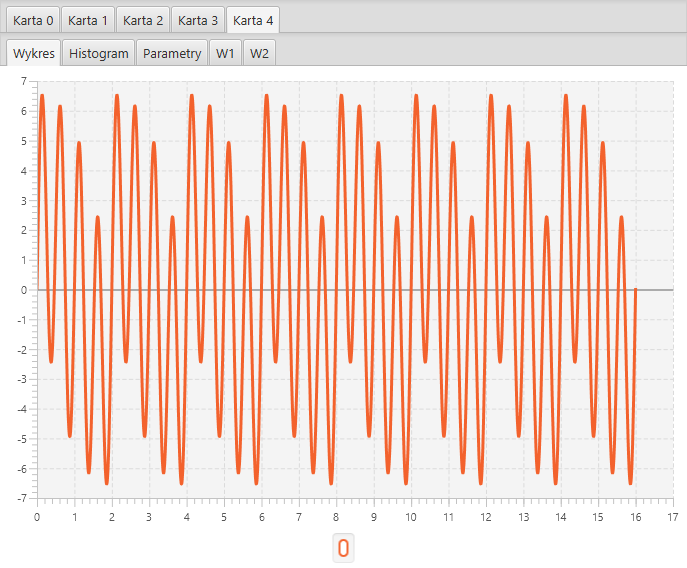
\includegraphics[width=\textwidth]{img/result/s2/data_134731.png}
                \caption{Wykres sygnału S2}
            \end{figure}
            \newpage

            \subsubsection{Dyskretna tranformacja Fouriera z definicji} {

                \begin{figure}[H]
                    \centering
                    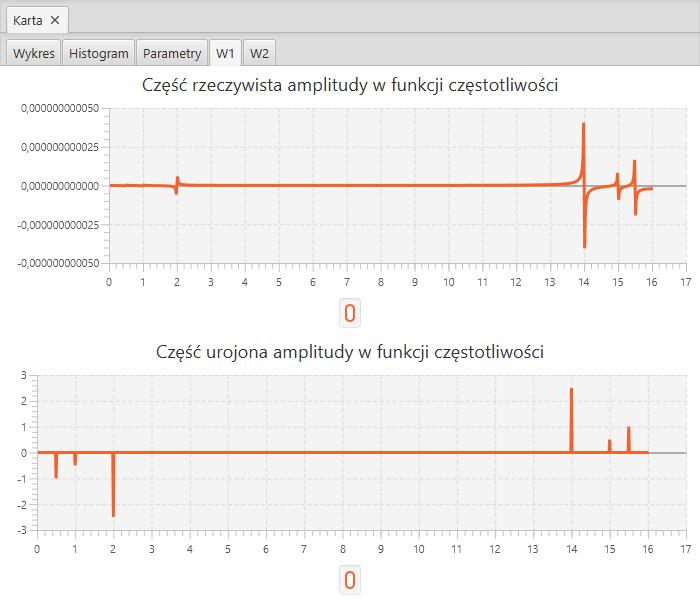
\includegraphics[width=0.65\textwidth]{img/result/s2/01/W1_draw_1_sinus_sampling_trans_s2_data_205737.png}
                    \caption{Wykresy}
                \end{figure}

                \begin{figure}[H]
                    \centering
                    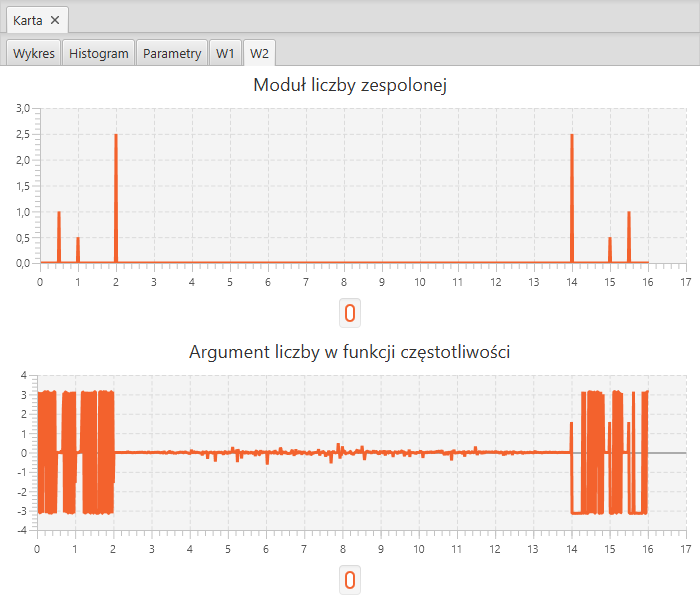
\includegraphics[width=0.65\textwidth]{img/result/s2/01/W2_draw_1_sinus_sampling_trans_s2_data_205737.png}
                    \caption{Wykresy}
                \end{figure}

                Czas wykonania obliczeń (s): 0.667
            }
            \newpage

            \subsubsection{Dyskretna tranformacja Fouriera wariant szybki in situ} {

                \begin{figure}[H]
                    \centering
                    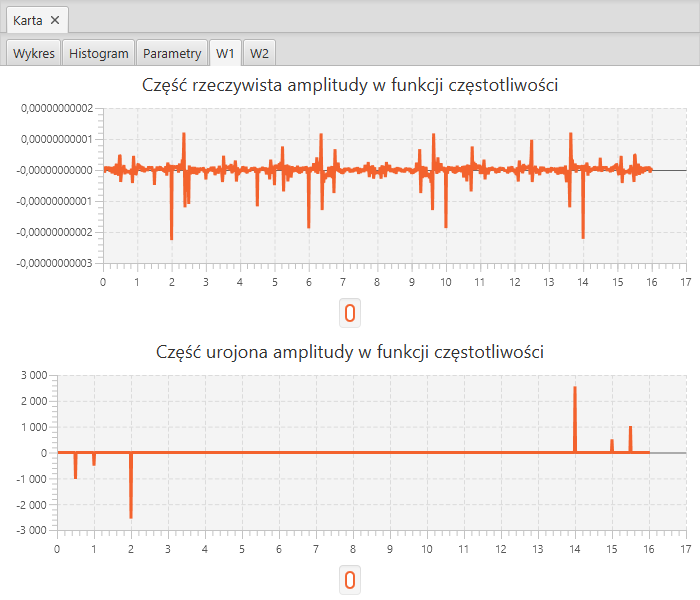
\includegraphics[width=0.65\textwidth]{img/result/s2/02/W1_draw_2_sinus_sampling_trans_s2_data_205743.png}
                    \caption{Wykresy}
                \end{figure}

                \begin{figure}[H]
                    \centering
                    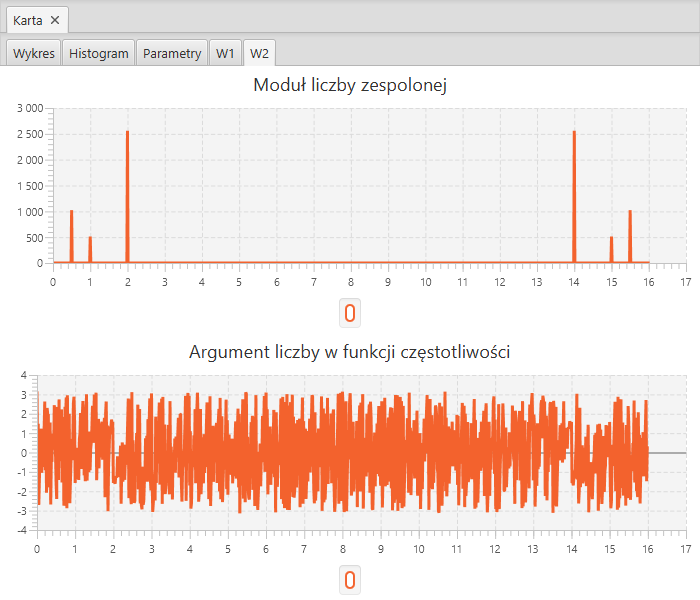
\includegraphics[width=0.65\textwidth]{img/result/s2/02/W2_draw_2_sinus_sampling_trans_s2_data_205744.png}
                    \caption{Wykresy}
                \end{figure}

                Czas wykonania obliczeń (s): 0.064
            }
            \newpage

            \subsubsection{Dyskretna tranformacja Fouriera wariant szybki rekurencyjny} {

                \begin{figure}[H]
                    \centering
                    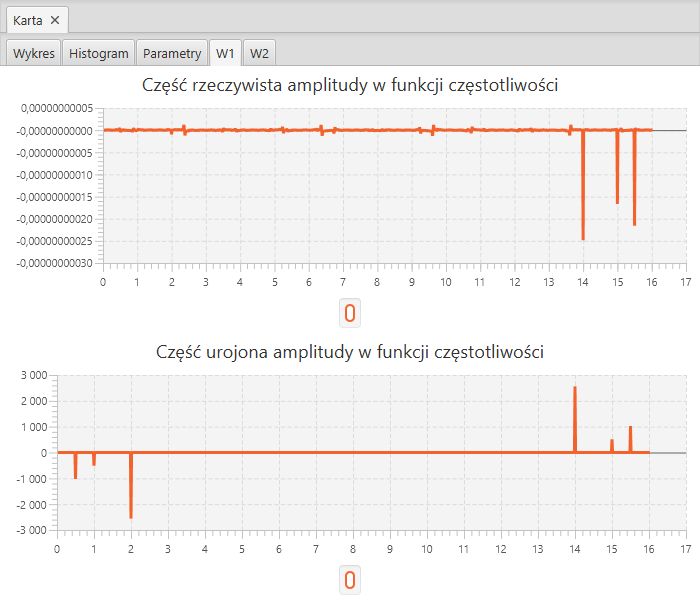
\includegraphics[width=0.65\textwidth]{img/result/s2/03/W1_draw_3_sinus_sampling_trans_s2_data_205751.png}
                    \caption{Wykresy}
                \end{figure}

                \begin{figure}[H]
                    \centering
                    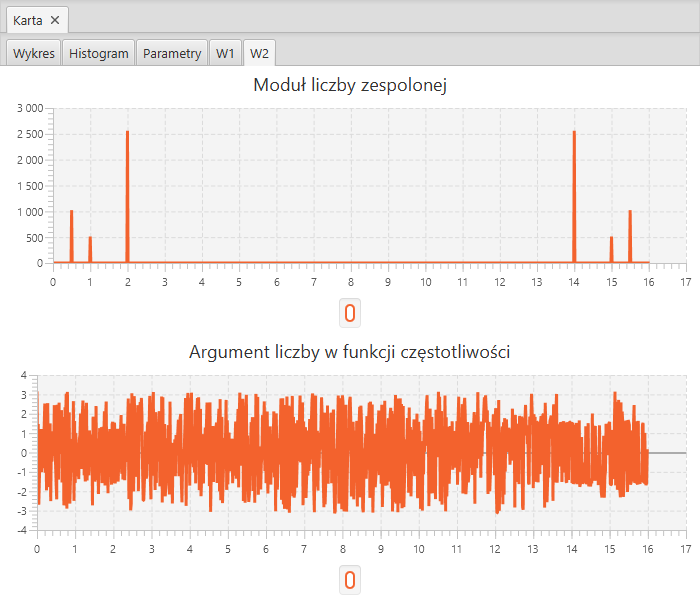
\includegraphics[width=0.65\textwidth]{img/result/s2/03/W2_draw_3_sinus_sampling_trans_s2_data_205752.png}
                    \caption{Wykresy}
                \end{figure}

                Czas wykonania obliczeń (s): 0.945
            }
            \newpage

            \subsubsection{Transformacja kosinusowa z definicji} {

                \begin{figure}[H]
                    \centering
                    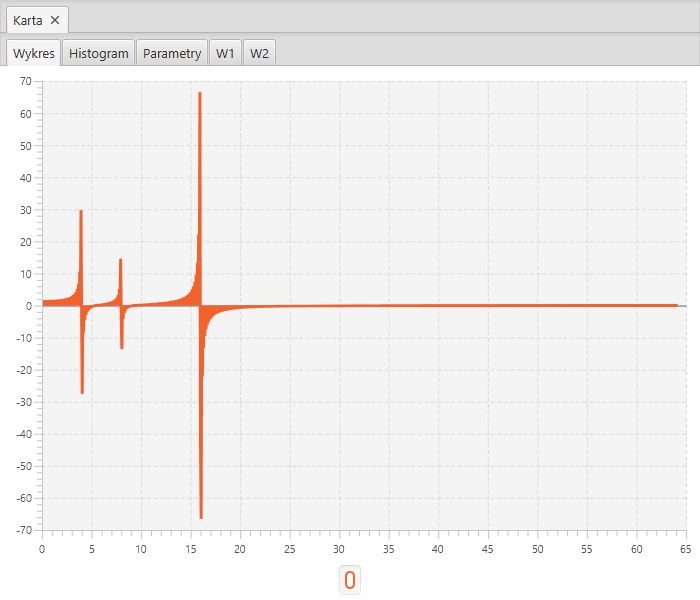
\includegraphics[width=\textwidth]{img/result/s2/04/data_draw_4_sinus_sampling_trans_s2_data_205806.png}
                    \caption{Wykresy}
                \end{figure}

                Czas wykonania obliczeń (s): 0.123
            }
            \newpage

            \subsubsection{Transformacja kosinusowa wariant szybki} {

                \begin{figure}[H]
                    \centering
                    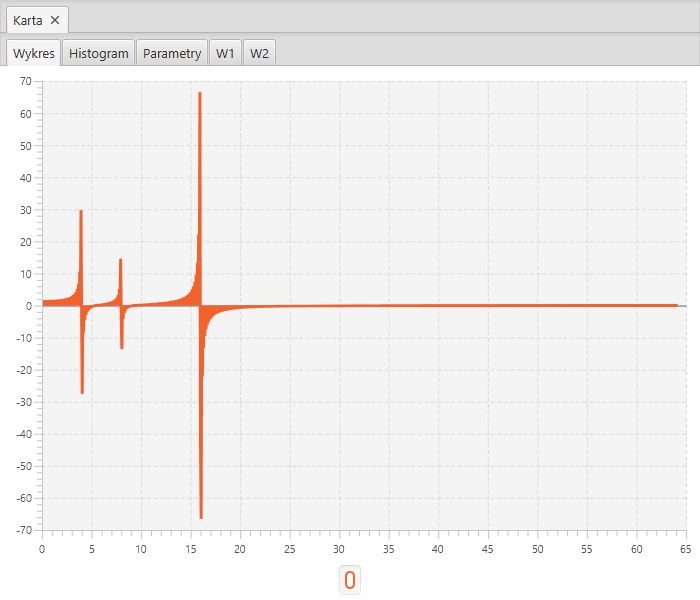
\includegraphics[width=\textwidth]{img/result/s2/05/data_draw_5_sinus_sampling_trans_s2_data_205820.png}
                    \caption{Wykresy}
                \end{figure}

                Czas wykonania obliczeń (s): 0.051
            }
            \newpage

            \subsubsection{Transformacja Walsha-Hadamarda z definicji} {

                \begin{figure}[H]
                    \centering
                    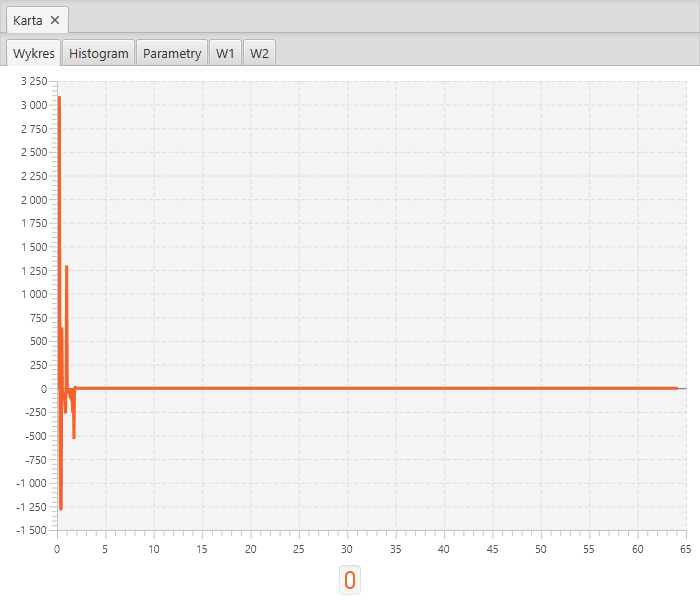
\includegraphics[width=\textwidth]{img/result/s2/06/data_draw_6_sinus_sampling_trans_s2_data_205829.png}
                    \caption{Wykresy}
                \end{figure}

                Czas wykonania obliczeń (s): 0.037
            }
            \newpage

            \subsubsection{Transformacja Walsha-Hadamarda wariant szybki} {

                \begin{figure}[H]
                    \centering
                    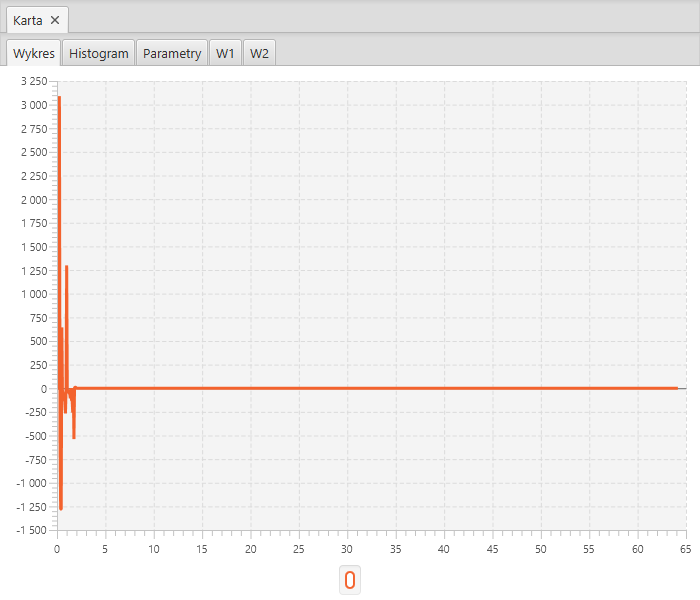
\includegraphics[width=\textwidth]{img/result/s2/07/data_draw_7_sinus_sampling_trans_s2_data_205838.png}
                    \caption{Wykresy}
                \end{figure}

                Czas wykonania obliczeń (s): 0.001
            }
            \newpage

            \subsubsection{Transformacja falkowa wariant DB4} {

                \begin{figure}[H]
                    \centering
                    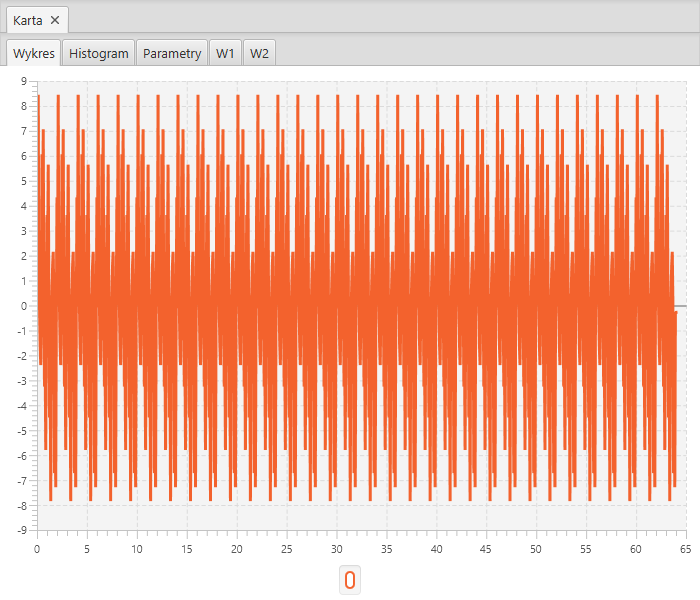
\includegraphics[width=\textwidth]{img/result/s2/08/data_draw_8_sinus_sampling_trans_s2_data_205848.png}
                    \caption{Wykresy}
                \end{figure}

                Czas wykonania obliczeń (s): 0.001
            }
            \newpage

        }
        \newpage
%--------------------------------------------------------------------------------------%
        \subsection{Sygnał S3} {

            \begin{figure}[H]
                \centering
                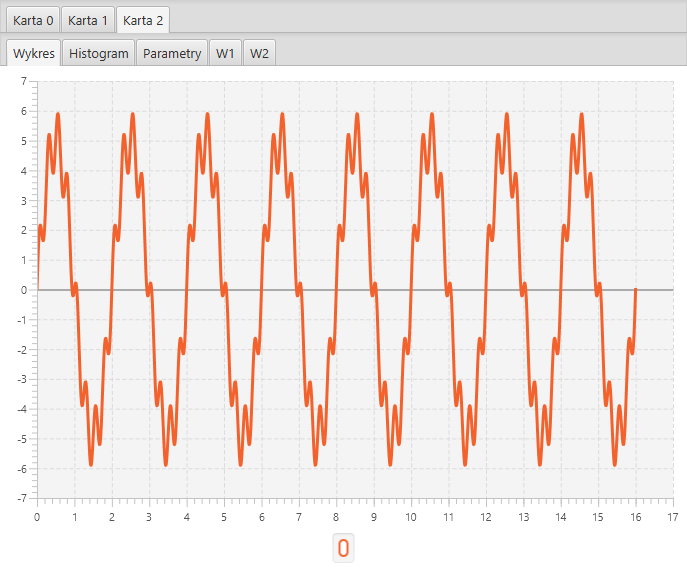
\includegraphics[width=\textwidth]{img/result/s3/data_134923.png}
                \caption{Wykres sygnału S3}
            \end{figure}
            \newpage

            \subsubsection{Dyskretna tranformacja Fouriera z definicji} {

                \begin{figure}[H]
                    \centering
                    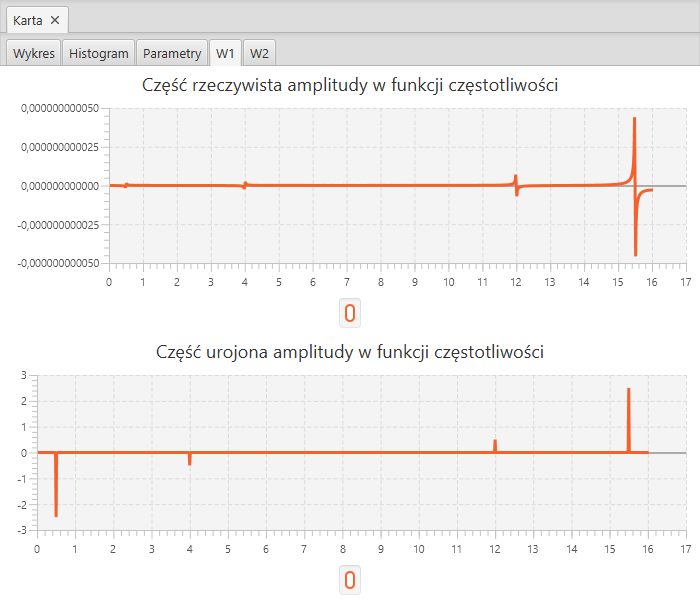
\includegraphics[width=0.65\textwidth]{img/result/s3/01/W1_draw_1_sinus_sampling_trans_s3_data_205855.png}
                    \caption{Wykresy}
                \end{figure}

                \begin{figure}[H]
                    \centering
                    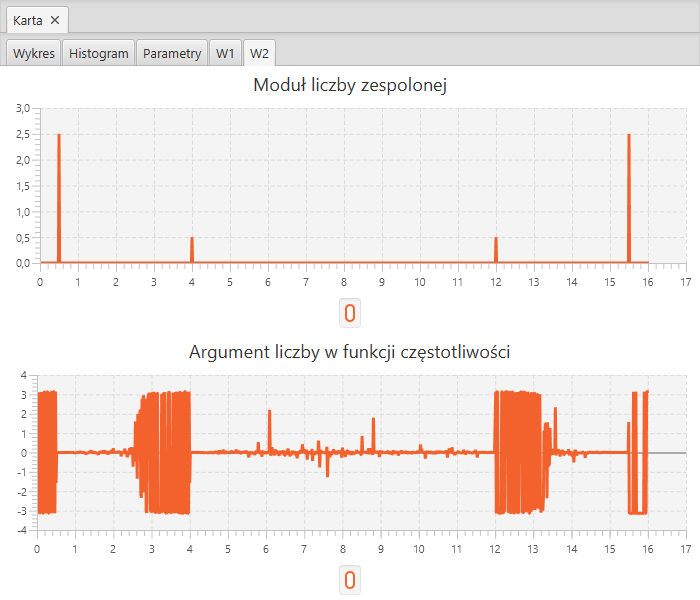
\includegraphics[width=0.65\textwidth]{img/result/s3/01/W2_draw_1_sinus_sampling_trans_s3_data_205856.png}
                    \caption{Wykresy}
                \end{figure}

                Czas wykonania obliczeń (s): 0.602
            }
            \newpage

            \subsubsection{Dyskretna tranformacja Fouriera wariant szybki in situ} {

                \begin{figure}[H]
                    \centering
                    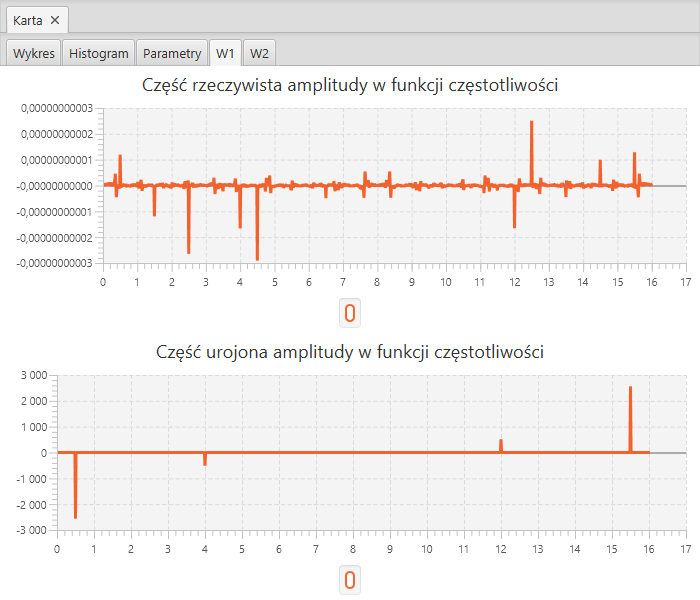
\includegraphics[width=0.65\textwidth]{img/result/s3/02/W1_draw_2_sinus_sampling_trans_s3_data_205903.png}
                    \caption{Wykresy}
                \end{figure}

                \begin{figure}[H]
                    \centering
                    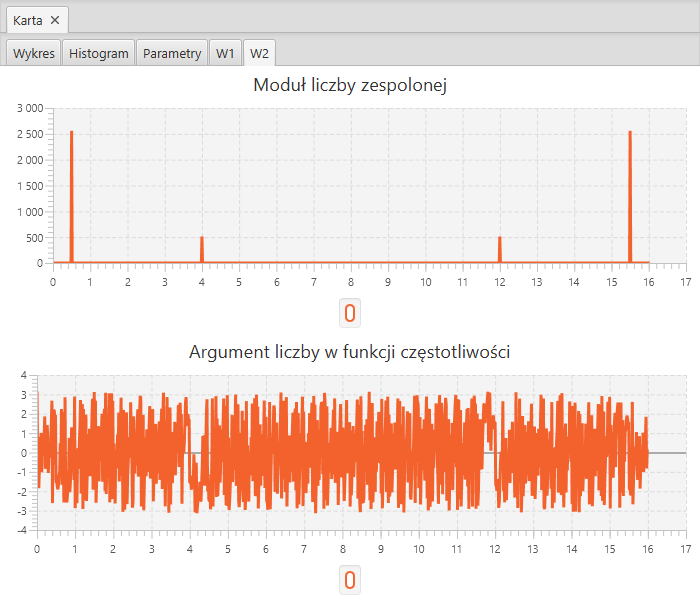
\includegraphics[width=0.65\textwidth]{img/result/s3/02/W2_draw_2_sinus_sampling_trans_s3_data_205904.png}
                    \caption{Wykresy}
                \end{figure}

                Czas wykonania obliczeń (s): 0.061
            }
            \newpage

            \subsubsection{Dyskretna tranformacja Fouriera wariant szybki rekurencyjny} {

                \begin{figure}[H]
                    \centering
                    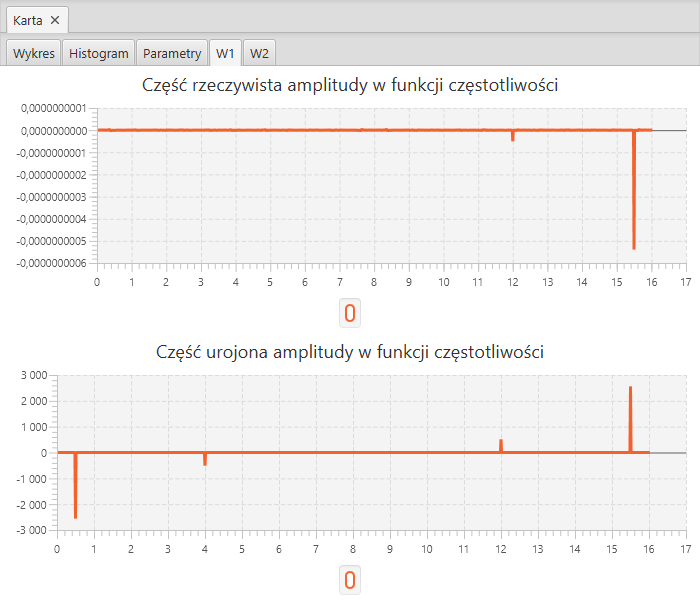
\includegraphics[width=0.65\textwidth]{img/result/s3/03/W1_draw_3_sinus_sampling_trans_s3_data_205911.png}
                    \caption{Wykresy}
                \end{figure}

                \begin{figure}[H]
                    \centering
                    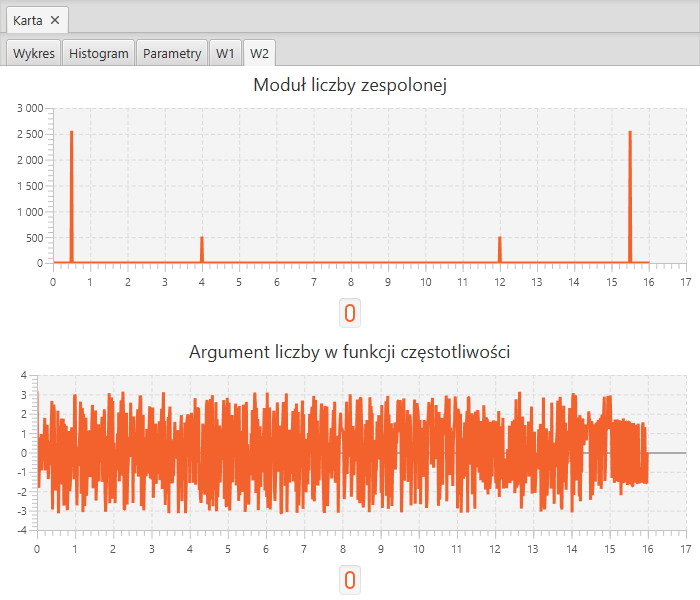
\includegraphics[width=0.65\textwidth]{img/result/s3/03/W2_draw_3_sinus_sampling_trans_s3_data_205911.png}
                    \caption{Wykresy}
                \end{figure}

                Czas wykonania obliczeń (s): 0.892
            }
            \newpage

            \subsubsection{Transformacja kosinusowa z definicji} {

                \begin{figure}[H]
                    \centering
                    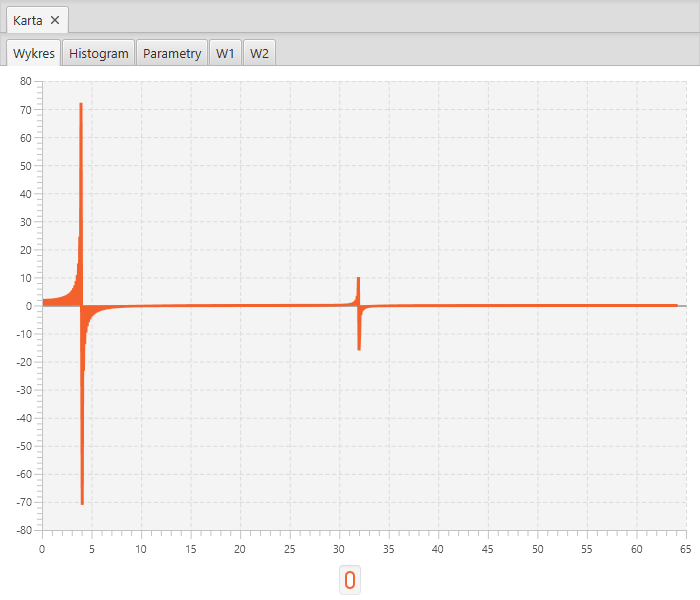
\includegraphics[width=\textwidth]{img/result/s3/04/data_draw_4_sinus_sampling_trans_s3_data_205925.png}
                    \caption{Wykresy}
                \end{figure}

                Czas wykonania obliczeń (s): 0.126
            }
            \newpage

            \subsubsection{Transformacja kosinusowa wariant szybki} {

                \begin{figure}[H]
                    \centering
                    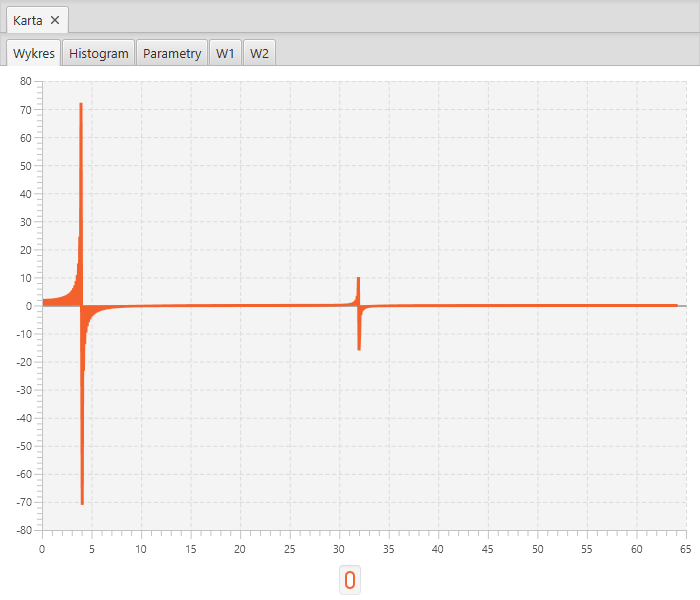
\includegraphics[width=\textwidth]{img/result/s3/05/data_draw_5_sinus_sampling_trans_s3_data_205938.png}
                    \caption{Wykresy}
                \end{figure}

                Czas wykonania obliczeń (s): 0.088
            }
            \newpage

            \subsubsection{Transformacja Walsha-Hadamarda z definicji} {

                \begin{figure}[H]
                    \centering
                    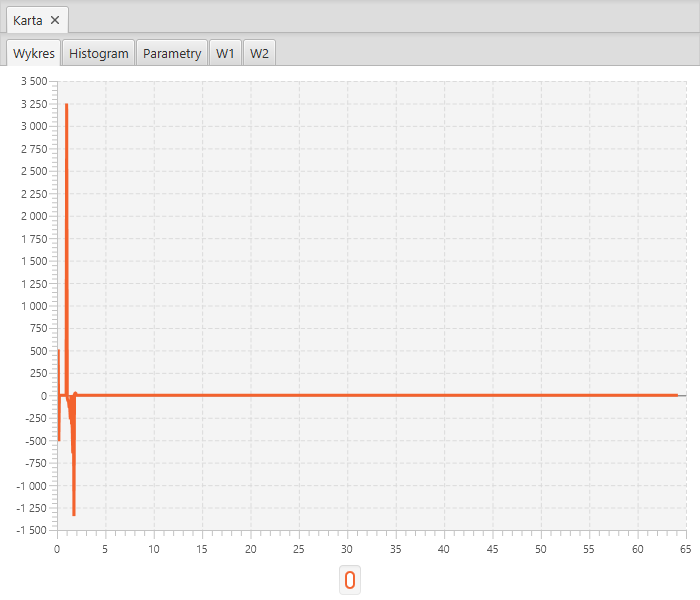
\includegraphics[width=\textwidth]{img/result/s3/06/data_draw_6_sinus_sampling_trans_s3_data_205946.png}
                    \caption{Wykresy}
                \end{figure}

                Czas wykonania obliczeń (s): 0.029
            }
            \newpage

            \subsubsection{Transformacja Walsha-Hadamarda wariant szybki} {

                \begin{figure}[H]
                    \centering
                    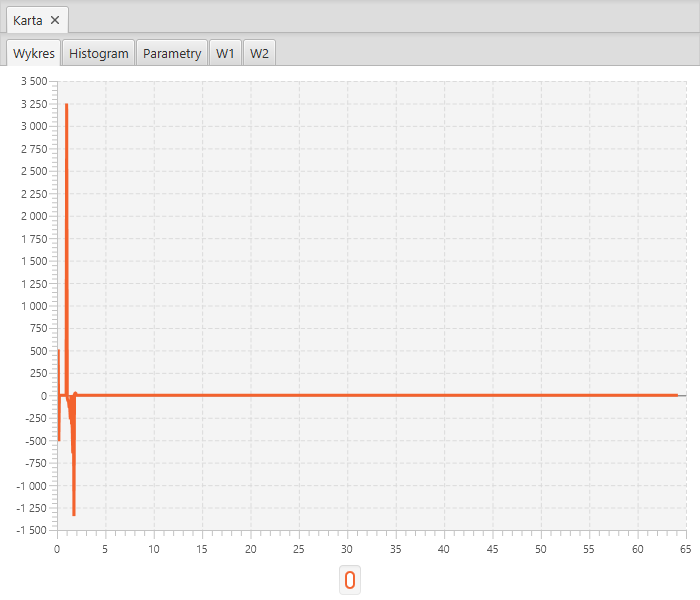
\includegraphics[width=\textwidth]{img/result/s3/07/data_draw_7_sinus_sampling_trans_s3_data_205955.png}
                    \caption{Wykresy}
                \end{figure}

                Czas wykonania obliczeń (s): 0.001
            }
            \newpage

            \subsubsection{Transformacja falkowa wariant DB4} {

                \begin{figure}[H]
                    \centering
                    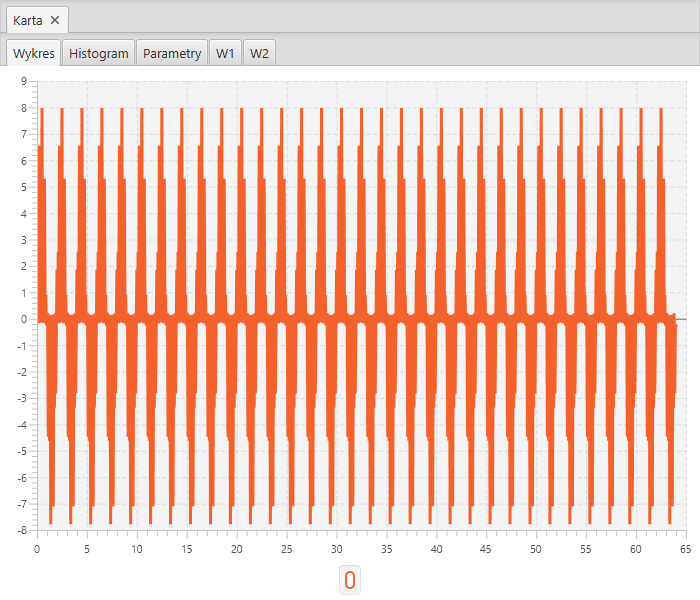
\includegraphics[width=\textwidth]{img/result/s3/08/data_draw_8_sinus_sampling_trans_s3_data_210006.png}
                    \caption{Wykresy}
                \end{figure}

                Czas wykonania obliczeń (s): 0.001
            }
            \newpage

        }
        \newpage

        \subsection{Tabela czasu wykonywania obliczeń w sekundach} {

            \begin{table}[H]
                \begin{tabular}{|l|l|l|l|}
                    \hline
                                                                                & S1        & S2     & S3        \\ \hline
                    Dyskretna tranformacja Fouriera z definicji                 & 0.71      & 0.667  & 0.602     \\ \hline
                    Dyskretna tranformacja Fouriera wariant szybki in situ      & 0.057     & 0.064  & 0.061     \\ \hline
                    Dyskretna tranformacja Fouriera wariant szybki rekurencyjny & 0.96      & 0.945  & 0.892     \\ \hline
                    Transformacja kosinusowa z definicji                        & 0.114     & 0.123  & 0.126     \\ \hline
                    Transformacja kosinusowa wariant szybki                     & 0.082     & 0.051  & 0.088     \\ \hline
                    Transformacja Walsha-Hadamarda z definicji                  & 0.033     & 0.037  & 0.029     \\ \hline
                    Transformacja Walsha-Hadamarda wariant szybki               & 0.001     & 0.001  & 0.001     \\ \hline
                    Transformacja falkowa wariant DB4                           & 0.001     & 0.001  & 0.001     \\ \hline
                \end{tabular}
            \end{table}
        }
        \newpage
    }
%--------------------------------------------------------------------------------------%
    \section{Dyskusja i wnioski} {
        Eksperymenty zostały podzielone na trzy grupy, każda grupa
        przedstawia wyniki transformacji jedego z sygnałów S1, S2 i
        S3. Większa liczba eksperymentów pozwala lepiej potwierdzić
        wysnuwane wnioski, które są w tym przypadku takie same, dla
        każdej serii doświadczeń.

        Jeżeli chodzi o wyniki transformacji, to wydają się one
        być poprawne dla wszystkich przeprowadzonych eksperymentów, w
        wynikach transformacji Fouriera, kosinusowej i
        Walsha-Hadamarda, zawsze można odnaleźć tyle składowych, ile
        rzeczywiście tworzyło transformowaną funkcję. I tak kolejno
        dla serii eksperymentów znaleziono 2, 3 i znowu 2 składowe.
        Warto jeszcze wspomnieć, że wyniki transformacji Fouriera,
        która była przeprowadzana różnymi metodami, również różnią się
        od siebie. Widać, że dla każdej z trzech metod część
        rzeczywista wyniku wygląda innaczej. Natomiast moduł zawsze
        wygląda tak samo i jako, że jest przeniesiony w dziedzinę
        częstotliwości a oś X odpowiednie przeskalowana, pozwala
        bezpośrednio odczytać, jakie częstotliwości składowe tworzyły
        transformowany sygnał. Oczywiście należy pamiętać, że druga
        połowa (w osi X) wykresu jest zawsze symetryczna do pierwszej
        i nie niesie dodatkowej informacji. Wyniki transformacji
        falkowej zawsze wyglądają zupełnie innaczej niż wyniki innym
        omawianych transformat, wygląda to z faktu, że transformacja
        ta w ogóle nie przenosi funkcji w dziedzinę częstotliwości
        tylko zostaje w dziedzinie czasu.

        Ostatnim rozważanym aspektem jest czas obliczeń. Pierwszym
        oczywistym wnioskiem potwierdzonym przez prawie wszystkie
        doświadczenia (poza rekurencyjną FFT) jest to, że algorytmy
        szybkie działają znacznie szybciej, niż algorytmy zbudowane na
        podstawie definicji. Widać to wyraźnie na przykładach
        transformacji Walsha-Hadamarda, kosinusowej i Fouriera (in
        situ). FFT (in situ) okazała się za każdym razem około
        dziesięciokrotnie szybsza niż transformacja z definicji. W
        przypadku transformacji kosinusowej jest to ok dwa razy
        szybciej a w przypadku transformacji Walsha-Hadamarda ponad
        trzydzieści razy. Warto zwrócić tutaj uwagę, że w ogóle
        transformacja falkowa okazała się najszybsza, druga w
        kolejności jest transformacja Walsha-Hadamarda, później
        transformacja kosinusowa, najwolniejsza natomiast jest
        transformacja Fouriera. Należy wziąc pod uwagę, że
        zależności pomiędzy czasem trwania różnych algorytmów zmienią
        się dla większej bądź mniejszej liczby próbek. Zysk czasowy,
        który otrzymujemy dla algorytmów szybkich, zawsze jest coraz
        bardzie zauważalny przy obliczeniach, na większej ilości
        danych. Ponadto trzeba wspomnieć, że czas obliczeń może
        zmieniać się w zależności od chwilowego obciążenia procesora
        komputera i konkretnych szczegółów implementacyjnych, które
        nie są charakterystyczne dla algorytmu ale dla danej jego
        implementacji. Jeżeli chodzi o FFT rekurencyjną, to mimo, iż
        algorytm ma oczywiście mniejszą złożoność niż algorytm z
        defnicji, to uzyskane czasy są tego samego rzędu a dokładnie
        to okazują się trochę dłuższa (o kilkadziesiąt procent). Jest
        to ciekawy przypadek potwierdzający, jak implementacja może
        wpłynąć na czas trwania danego algorytmu. W tym przypadku
        okazało się, że prawdopodobnie potrzeba alokacji nowej pamięci
        na każdym etapie obliczeń jest tak wymagająca czasowo, że
        wyniki są wolniejsze niż w przypadku algorytmu z definicji,
        mimo mniejszej złożoności obliczeniowej. Może też mieć na to
        wpływ potrzeba obliczania współczynników za każdym razem
        od nowa.
    }
%--------------------------------------------------------------------------------------%
    \renewcommand\refname{Bibliografia}
    \bibliographystyle{plain}
    \bibliography{bibliografia_wzor}

\end{document}
